\section{Evaluation}

\subsection{Experimental Setup}

The implementation mainly consists of two components; the test suite and the sketching algorithms. The entire code-base has been written in Python 3.8. All the tests were run on a 12-core Ryzen 3900 machine with a base clock of 3.1GHz and 32 GB RAM. However, only one core was utilized in running the tests. 

% The architecture of the benchmarking test suit is shown in Fig.~\ref{fig:test_suite}. It was designed in a modular way such that it permits easy addition of more test cases and graph sketches when necessary. 

% \begin{figure}[htbp]
%     \centerline{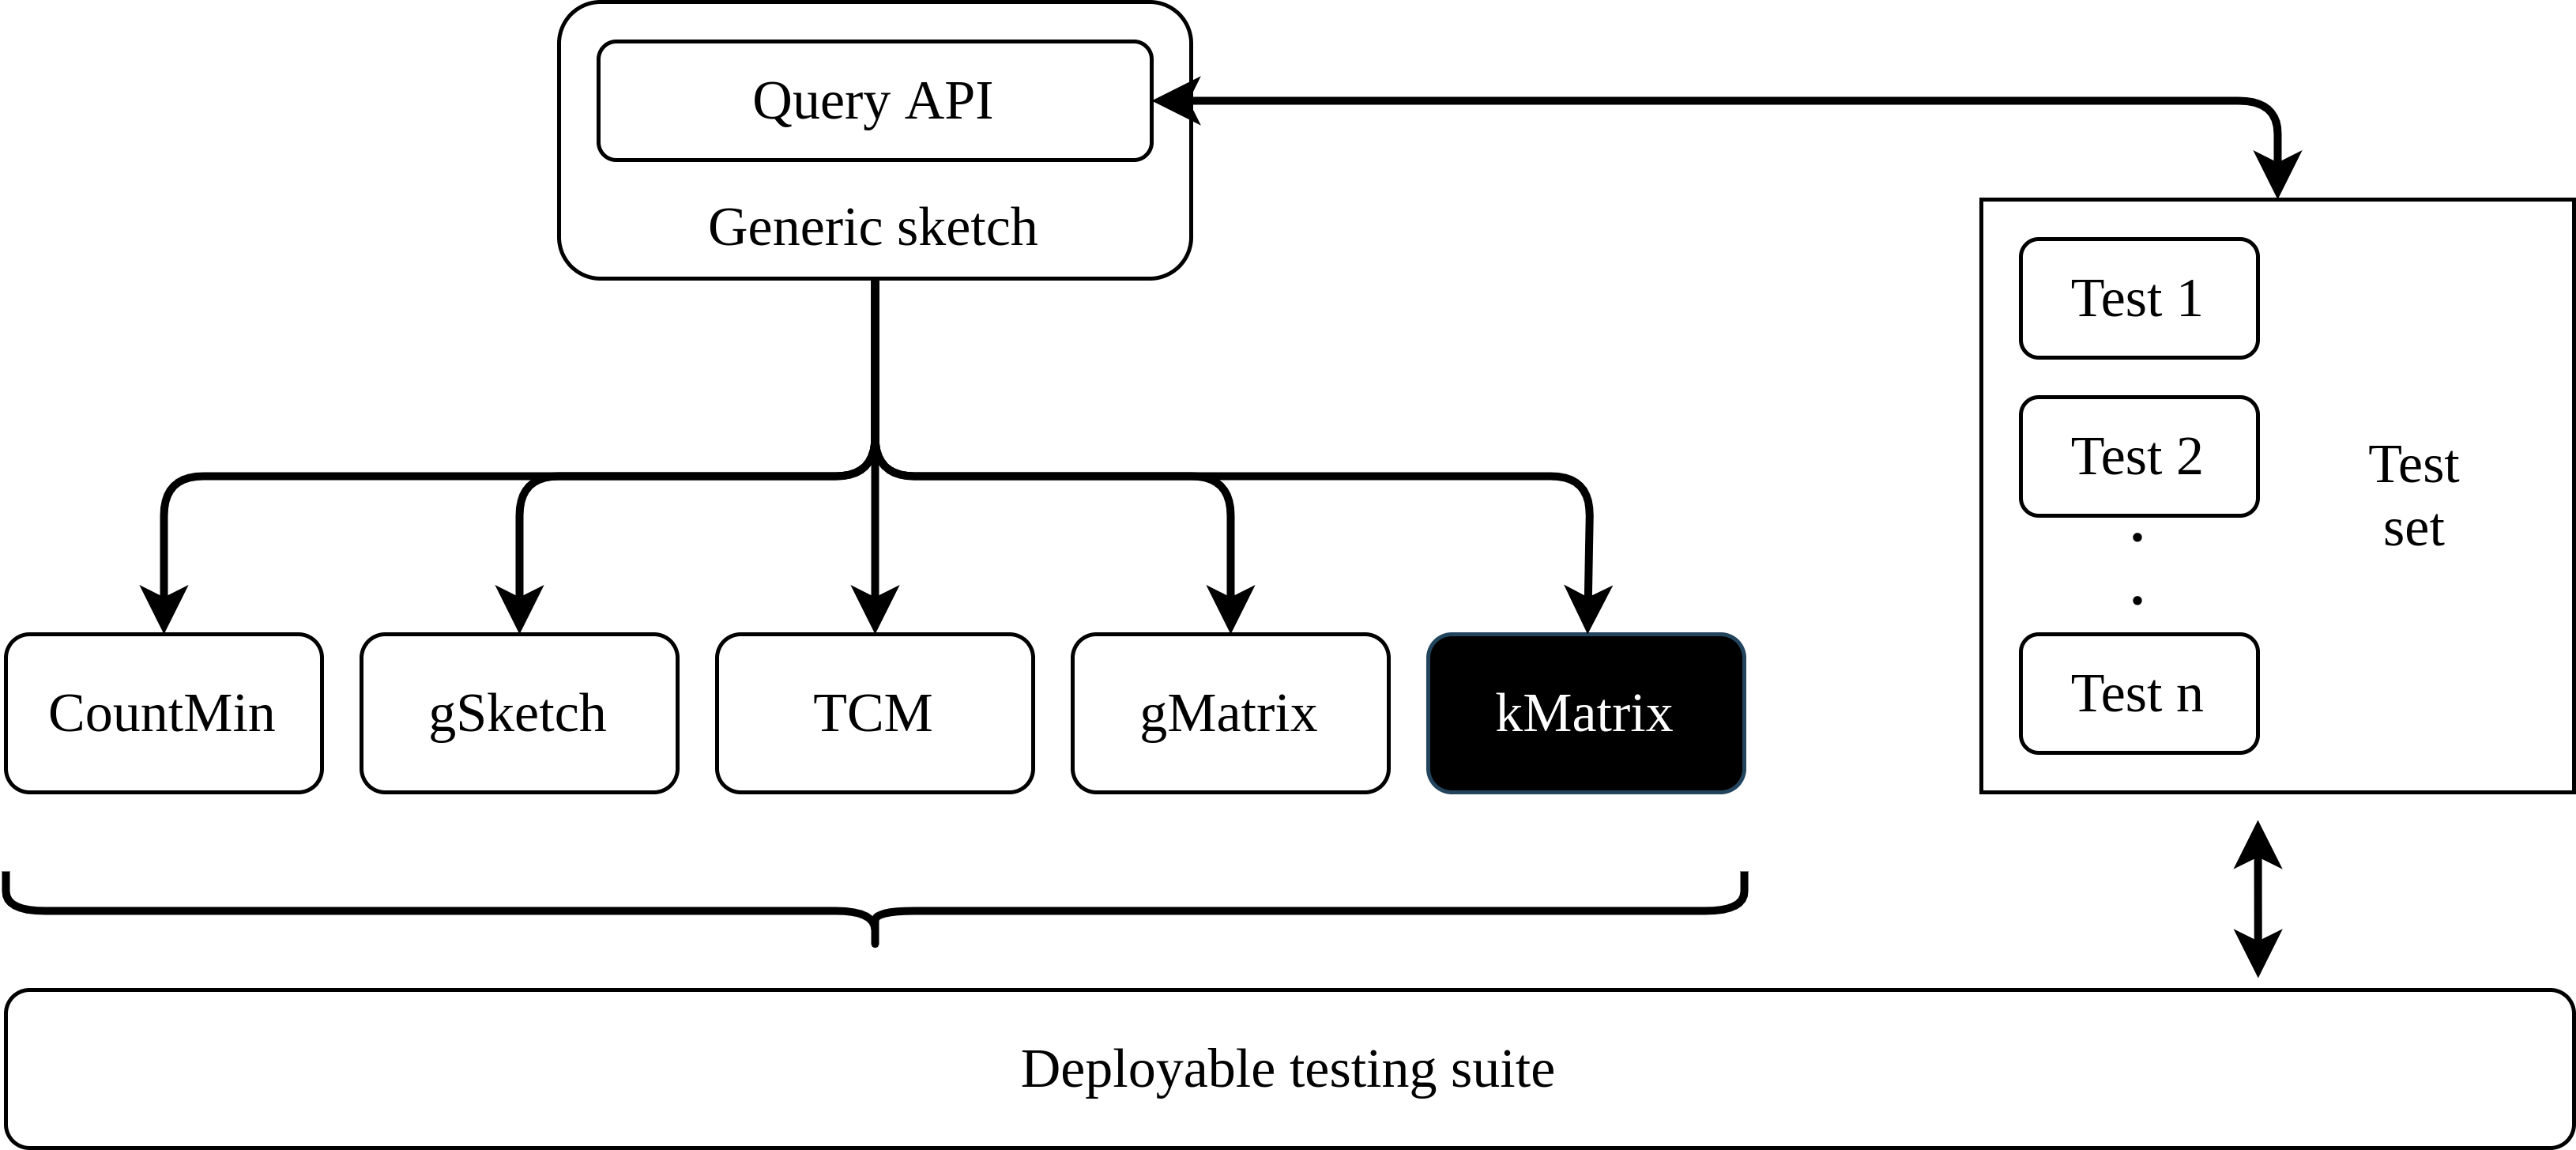
\includegraphics[width=0.5\textwidth]{img/test_suite.png}}
%     \caption{High level architecture of the test suite}
%     \label{fig:test_suite}
% \end{figure}

A sample of 30,000 edges has been extracted from relevant datasets for initializing kMatrix at the beginning of each experiment. This sample stream has been obtained using reservoir sampling. 

\subsection{Datasets}

3 datasets were chosen to carry out the benchmarking process in this research. These were chosen to represent different application domains. 

\paragraph{unicorn-wget\cite{DVN/5H4TDI_2018}}
unicorn-wget is a dataset created from capturing the packet information of the network activity of a simulated network. This dataset was created at Harvard University. The dataset consists of 5 parts. From them, Hour-Long Wget Benign Dataset (Base Graph) which consist of 17,778 nodes and 2,779,726 edges was chosen for the experiment. We filtered 10\% of the edges using reservoir sampling for our experiments. 

\paragraph{email-EuAll\cite{leskovec_graph_2007}}
This data was extracted using email data from a large European research institution. The dataset consists of emails sent out in a period of 18 months. Each data item contains sender, receiver and the time of the origination of each email. The dataset consisted of 265,214 nodes and 420,045 edges\cite{noauthor_snap_nodate_email}. 

% \paragraph{cit-HepPh\cite{leskovec_graphs_2005, gehrke_overview_2003}}
\paragraph{cit-HepPh\cite{gehrke_overview_2003}}
cit-HepPh citation graph is from the e-print arXiv regarding high energy physics phenomenology. It has 34,546 papers (nodes) and 421,578 citations (edges). We used the full dataset in our experiments. 

\subsection{Evaluation Metrics}
\label{section:design_evaluation_metrics}

\subsubsection{Average Relative Error (ARE)}
\label{section:metrics_are}

The average relative error is defined as,

\begin{equation}
    er(Q) =  \frac{\tilde{f}'(Q) - f(Q)}{f(Q)} = \frac{\tilde{f}'(Q)}{f(Q)} -1
\end{equation}

Given a set of m queries, $\{ Q_1 , ....., Q_m \}$, the average relative error is defined by taking the average of the relative error of all queries $Q_i$ for \(i \in [1,m]\).

\begin{equation}
    e(Q) =  \frac{\sum_{i=1}^{k} er(Q_i)}{m}
\end{equation}

\subsubsection{Number of Effective Queries (NEQ)}
\label{section:metrics_neq}

A query is said to be effective if the error, $\tilde{f}'(Q) - f(Q), \leq G_0$,  where $G_0$ is a predefined value. The number of effective queries is defined as,

\begin{equation}
    g(Q) =  |\{\,q\, | \, (\tilde{f}'(q) - f(q)) \leq G_0, \,q\, \epsilon \,Q\}|
\end{equation}

% This can also be expressed as a percentage of effective queries (PEQ).

% \begin{equation}
%     g(Q) =  \frac{\left | \{\,q\, |   \left |\tilde{f}'(q) - f(q)\right | \leq G_0, \,q \, \epsilon  \,Q\} \, \right|}{|Q|}*100
% \end{equation}
